\section{Versuchsaufbau/-durchführung}
In diesem Abschnitt werden nun die verwendeten Brückenschaltungen aufgeführt. \\
Zur Bestimmung eines unbekannten ohmschen Widerstandes, wird die Wheatonsche Brücke
benutzt (Abbildung \ref{fig: wheaton}).
\begin{figure}
  \centering
  \fbox{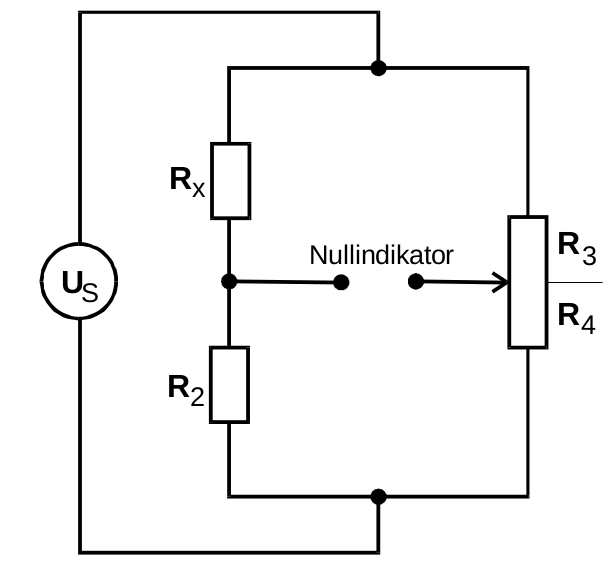
\includegraphics[width = 5cm]{pics/wheaton.png}}
  \caption{Wheatonsche Brückenschaltung\cite{anleitung302}}
  \label{fig: wheaton}
\end{figure}
Der Zusammenhang \eqref{eq: widerstandsbedingungen} vereinfacht sich in diesem Fall zu:
\begin{equation}
  R_{\symup{X}} = R_2 \frac{R_3}{R_4}
\end{equation}
Das Verhältnis $R_3 / R_4$ ist durch ein Potentiometer realisiert. Um eine Fehlerrechnung durchführen
zu können, wird der Widerstand drei mal varriert und jeweils die entsprechenden Werte für $R_3$, die
zum Verschwinden der Brückenspannung führen, aufgenommen. Als Nullindikator wird ein Oszilloskop verwendet. \\
Nach dem selben Prinzip werden die Kapazität eines Kondensators und dessen Wirkwiderstand bestimmt. Der Aufabu
der Kapazitätsmessbrücke ist in Abbildung \ref{fig: brücke} dargestellt.
\begin{figure}
  \centering
  \fbox{\includegraphics[width = 5cm]{pics/kap_brücke.png}}
  \caption{Kapazitätsmessbrücke\cite{anleitung302}}
  \label{fig: kapazität}
\end{figure}
Hierbei wird zunächst von einem idealen Kondensator ausgegangen, $R_x$ bzw. $R_2$ also aus der Schaltung entfernt. Für die
Kapazität $C_{\symup{X}}$ gilt in diesem Fall:
\begin{equation}
  C_{\symup{X}} = C_2 \frac{R_4}{R_3}
  \label{eq: Cx}
\end{equation}
Zur Bestimmung von $R_{\symup{X}}$ einer realen Kapazität wird als weiteres Stellglied der Variable Widerstand $R_2$ in Reihe mit dem Kondesator $C_2$
geschaltet. Als weitere Bedingung neben \eqref{eq: Cx} für die Nullmethode ergibt sich:
\begin{equation}
  R_{\symup{X}} = R_2\frac{R_3}{R_4}
  \label{eq: Rx}
\end{equation}
Die Messung einer realen Induktivität wird zunächst mit einem Aufbau der Form \ref{fig: induktivität} durchgeführt.
Hier gelten als Bedingungen für $U_{\symup{Br}} = 0$:
\begin{align}
  \begin{aligned}
    R_{\symup{X}} &= R_2\frac{R_3}{R_4} \\
    L_{\symup{X}} &= L_2\frac{R_3}{R_4}
  \end{aligned}
  \label{eq: Lx}
\end{align}
\begin{figure}
  \centering
  \fbox{\includegraphics[width = 5cm]{pics/ind_brücke.png}}
  \caption{Induktivitätsmessbrücke\cite{anleitung302}}
  \label{fig: induktivität}
\end{figure}
Anschließend geschieht die Induktivitätsmessung erneut mittels einer Maxwell-Brücke (siehe Abbildung \ref{fig: maxwell}).
\begin{figure}
  \centering
  \fbox{\includegraphics[width = 5cm]{pics/max_brücke.png}}
  \caption{Maxwell-Brücke\cite{anleitung302}}
  \label{fig: maxwell}
\end{figure}
Hierbei sind nun dei Wiederstände $R_3$ und $R_4$ als unabhängige Stellglieder eingebaut. Die Bedingungen für die Nullmethode lauten
bei diesem Aufbau:
\begin{align}
  \begin{aligned}
    R_{\symup{X}} &=\frac{R_2 R_3}{R_4} \\
    L_{\symup{X}} &= R_2 R_3 C_4
  \end{aligned}
  \label{eq: Lx_maxwell}
\end{align}
